% !TeX root = ../main.tex

\chapter{神经网络}
\label{chap:NN}

为了识别信号中的位移喷注(displaced jets)与类标准模型(SM-like)喷注以及由束流背景(BIB)产生的伪喷注,训练了一个逐喷注(per-jet)的神经网络(NN)。
该神经网络在隐藏区域(Hidden Sector)模型信号、标准模型多喷注(SM Multi-jets)以及 BIB 的混合样本上进行训练。
神经网络的输入变量为与每个喷注相关的低级特征,涵盖整个 ATLAS 探测器的信息,包括径迹、量能器以及 μ 子谱仪相关信息。
训练前对每个变量进行了预处理,以确保神经网络训练的最优效果。
NN 的主体结构选用基于 Transformer\cite{vaswani2023attentionneed} 的图神经网络(Graphic Neural Network, GNN)。
训练采用 Pytorch\cite{paszke2019pytorchimperativestylehighperformance} 框架,
并使用 Optuna\cite{akiba2019optunanextgenerationhyperparameteroptimization} 框架进行超参数(hyperparameter)优化。
训练结果经过评估以排除过拟合现象,并在所用信号样本上相较于此前的网络性能有所提升。

训练使用的信号区域(signal region)数据集包括来自探测器的 BIB 数据(见\autoref{sec:detector_data})
和信号与标准模型多喷注(简记为 QCD)模拟数据(见\autoref{sec:MC})。
训练中使用的喷注均为 clean 喷注,其定义见\autoref{sec:jet_preselection}。
信号喷注为隐藏区域(Hidden Sector)模型中由一系列不同的$m_\Phi$、$m_s$、$c\tau$参数生成的模拟数据,
其中 $m_\Phi$ 为中介粒子质量,$m_s$ 为 LLP 的质量,$c\tau$ 为 LLP 衰变长度。
训练阶段仅使用事件编号为奇数的信号事件,偶数编号的事件则用于后续分析流程,以避免因数据重叠而引发的偏差,确保最终结果的客观性和可信度。
对于 QCD 喷注,训练样本来自 JZ2W、JZ3W 和 JZ4W 样本,
这些样本覆盖了 \pt 范围为 60 GeV 至 800 GeV 的双喷注(dijet)事件,叠加的 pileup 喷注将该范围的下界扩展至 40 GeV。
BIB 喷注训练样本选取触发 HLT CalRatio 触发器但未通过 HLT BIB 抑制算法的事件。
随后通过 $\Delta R$ 匹配离线喷注与触发喷注,匹配成功并满足公共选择条件的喷注被标记为 BIB 喷注。

为了进行补充训练以及计算本分析中使用的机器学习方法的系统不确定性,需要在数据和 MC 模拟中定义一个控制区域(control region)。
控制区域中所选样本具有统一的筛选条件(见\autoref{cpm:CR_jet_selection}),以确保喷注来源于相同的产生机制,并覆盖相同的运动学范围。
控制区域数据包括探测器数据和 QCD 模拟数据。

信号区域上定义的主数据集总计有 2.09M jets,其中 766k jets 属于信号集、660k jets 属于 QCD 集、660k jets 属于 BIB 集。
控制区域上定义的补充数据集总计有 449k jets,其中 223k jets 属于 MC 模拟、226k jets 属于探测器。

由于信号与背景喷注可通过 ATLAS 探测器的各个子系统加以刻画,因此神经网络也应当充分利用来自各子探测器的信息。
NN 输入变量的概述如下(详见\autoref{cpm:NN_variables}):
\begin{itemize}
    \item 位于喷注轴线 $\Delta R < 0.2$ 范围内的径迹的空间位置、动量、碰撞参数(impact parameter)和径迹拟合质量参量(quality variables);
    \item 与喷注相关联的拓扑集团(topo-clusters) 的动量、时间信息和空间位置;
    \item 喷注在电磁量能器与强子量能器各层的能量沉积比例;
    \item 位于喷注 $\Delta \phi < 0.2$ 范围内的μ子段(muon segment)的空间与时间信息;
    \item 喷注本身的动量与空间位置。
\end{itemize}

训练前对所有输入变量进行预处理,调整变量分布使得各变量的均值为0、标准差为1,以加快训练收敛速度。
预处理完成后,喷注输入至神经网络,网络输出对应于信号、QCD 或 BIB 的预测权值。


\section{网络结构}
\begin{figure}[ht]
    \centering
    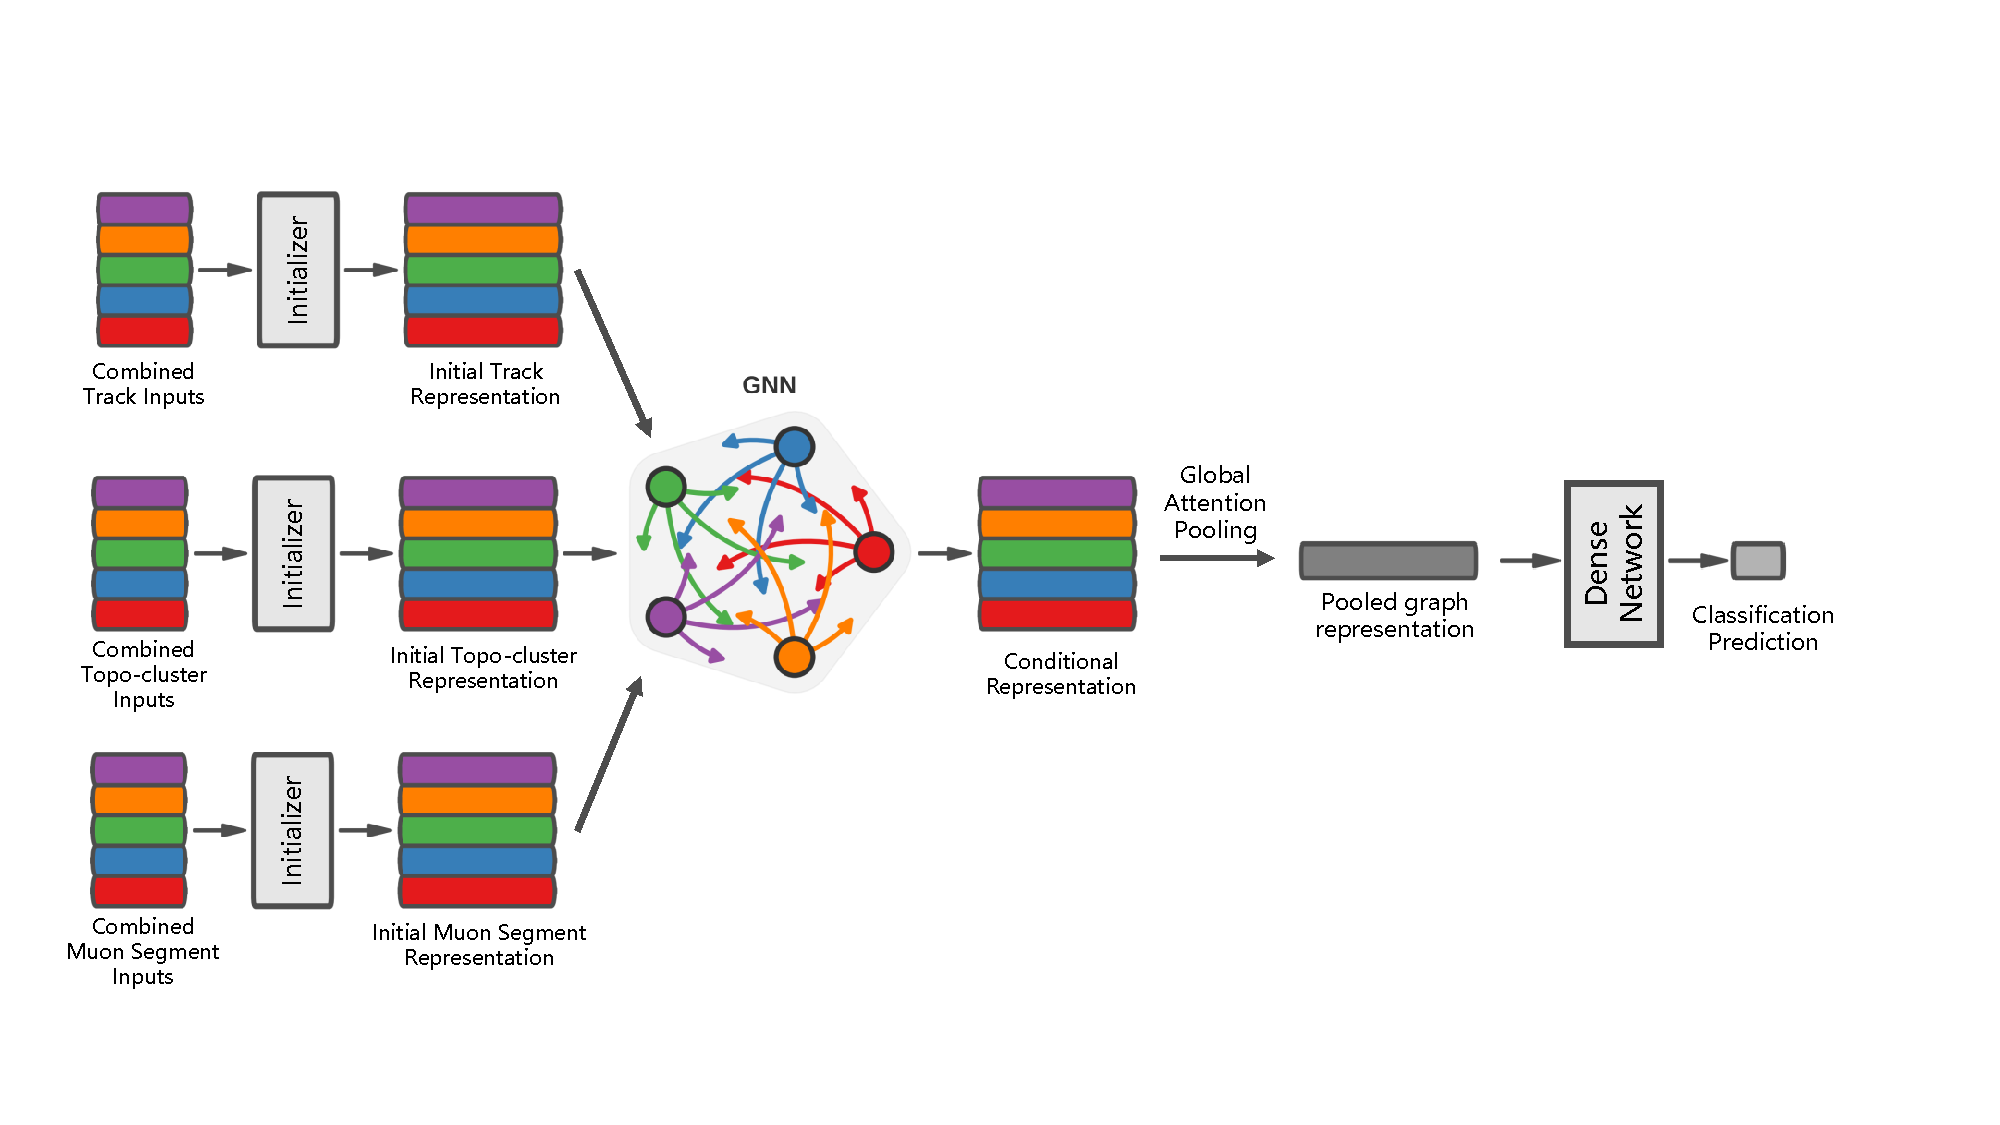
\includegraphics[width=\textwidth]{CalRatio_GNN_Architecture.pdf}
    \caption{GNN 网络结构示意图}
    \label{fig:CalRatio_GNN_Architecture}
\end{figure}

逐喷注神经网络的结构如\autoref{fig:CalRatio_GNN_Architecture} 所示。
来自径迹、量能器和 μ 子谱仪的输入变量被分别输入至用于初始化的子网络(initializer)中,得到维度相同的向量表示。
每个向量表示作为全连接图神经网络的节点,根据节点之间的相关性计算注意力权重作为边值。
然后利用 Transformer 机制更新节点表示得到下一层 GNN,最后一层 GNN 的所有节点经过池化(pooling)得到单向量特征表示。
将该特征表示传入全连接层分类器,得到最终分类的预测值。

基于 Transformer 的 GNN 兼顾了节点自身的特征提取(通过自注意力机制)和节点间的相关性(通过注意力边值),
获得了更好的特征提取与表示能力,得到了相较于卷积神经网络(CNN)\cite{} 更好的性能(见\autoref{})。


\section{训练方法}
此外,还在神经网络输出后添加了一个对抗网络(adversarial network),该网络用于在控制区中学习区分模拟喷注与真实数据喷注的特征,并将此反馈至主网络以抑制数据与 MC 的不一致性。这一对抗训练显著降低了数据与 MC 模型之间的差异,效果可见图 10 与图 11 中 BIB 分数的比较。网络结构图与对抗训练流程可见图 9。


\section{结果}
最终训练效果可见图 12--14,分数越低表明被标记为该类别喷注的可能性越低,分数接近 1 则表示为该类别喷注的置信度越高。训练约经历 50 个 epoch(遍历完整训练集)收敛。有关神经网络输入建模的不确定性的系统评估流程见附录 B.9。

